\documentclass[12pt, letterpaper]{article}
\usepackage[utf8]{inputenc}
\usepackage{graphicx}

\usepackage[usenames,dvipsnames]{color}
\newcommand{\todo}[1]
  {{\scriptsize \textbf{\color{red} {#1}}}}
  
   
\title{Challenges faced in the process of knowledge transfer in an industrial environment}
\author{Mauricio Soto\\
mauriciosoto@cmu.edu
}
\date{Fall 2017}
 
\begin{document}
 
\begin{titlepage}
\maketitle


\begin{abstract}
I analyze the knowledge transfer process I went through in my previous experiences in industrial environments.
I contrast and compare the four different industrial experiences I had before joining the PhD program and 
how knowledge transfer played an important role in my learning process for each of these companies.
I discuss how the knowledge transfer process was handled in different ways in the different contexts I took part
of and how the resources and mechanisms companies have to handle knowledge transfer have an impact in the 
amount of time needed to be spent by both the newcomers and the mentors to understand the code base. 
\end{abstract}
\end{titlepage}
 
\section{Introduction}

Knowledge is of utmost importance in current enterprises. It is one of the key assets to maintain competitiveness
and the role that knowledge plays in the current market is continuously growing. 
It is critical for companies to be able to maintain, increase and manage their knowledge in the face 
of constant change. To sustain competitive advantages, companies must assess their knowledge resources and 
establish their knowledge strategy~\cite{civi00}. In this context, the value of knowledge transfer 
becomes a decisive factor.

Knowledge transfer is a particularly challenging problem because of the characteristics of
knowledge itself. Knowledge is distributed, ambiguous and 
disruptive~\cite{Newell06}, making its transfer a very
slow and troublesome process. 
In the context of the software industry, this knowledge includes aspects such as: specific training in tools and standard procedures used by the enterprise, as well as the
business logic required to understand the proper use and requirements of the product being built
in the branch. The social problems that convey this process are also part of the challenges faced during the 
knowledge transfer process such as resistance to power-knowledge
shifts or close-mindedness.

A clear example when substantial knowledge needs to be transfered is when an enterprise opens a new branch.
Owning branches in different locations enables a pool of resources that enterprises would not be able
to obtain otherwise, such as special talents, legal benefits and financial gain~\cite{ceruttia07}. However, 
opening a new branch is accompanied by a set of challenges inherent to a process of this nature, such as 
difficulties in communication among team members distributed in different locations, 
cultural and language barriers, and transmitting the knowledge, culture, and mechanisms necessary for the 
coworkers in the new branch to perform their tasks adequately.

I have had the opportunity to work with very diverse contexts of knowledge and culture transfer in 
an industrial environment. I will compare and contrast my experiences, with a slight emphasis on the 
latest experience I had before joining the PhD program. A large well-known enterprise was 
opening a new branch in Costa Rica and was starting to face the challenges this process encompasses.  


\section{Knowledge management and transfer}
Knowledge is one of the most important organizational resources current enterprises possess.
The transfer of this knowledge is a key process to maintain, augment and
make proper use of that knowledge base. 
There are continuous efforts to creating ways of preserving knowledge in society and software 
companies are not an exception. In an enterprise environment, the concept of Knowledge Management
has gained importance in the last decades, as the process of dealing with the management 
of knowledge and its related activities which encompasses 
the following goals~\cite{wiig97}: 
\begin{itemize}
\item To make the enterprise act as intelligently as possible to secure its viability and overall success, and
\item To otherwise realize the best value of its knowledge assets
\end{itemize}

Organizing the process of passing down knowledge has noticeable gains in times
when knowledge is an increasingly important asset. Some of the benefits that come from proper management and transfer of knowledge are: Financial
Value, Operational Benefits, Business process improvement and Culture~\cite{ibrahim09}. These translate into concrete assets such as
improvements in cost, quality, cycle time, lead time, no need to reinvent the wheel, decision making and resolved complaints.

Learning is tightly connected to the knowledge transfer
process, and the learning capabilities of teams and individuals play an important role in 
this process.
There two kinds of knowledge: When you learn about something, referred to as explicit 
knowledge, and when you learn to do something, called tacit knowledge~\cite{cook99}. 
In the case of knowledge transfer in a industrial environment, collaborators need both, 
learning about (cognitive learning) and learn to do (behavioral learning).

When newcomers join a software project in an industrial environment, they find themselves in a project
landscape and they must become familiar with several features of this landscape.
There are three primary factors that impact the 
success newcomers have when facing a project landscape: early experimentation, internalizing structure
and culture, and progress validation~\cite{Dagenais10}.

The knowledge transfer process in an industrial context can take mainly two forms. It can be, for example,
face-to-face interactions between one or several apprentices and a mentor, or it can take the form of documentation 
(i.e. internal comments in the code, external documentation, educational videos, directives, etc). 

For the 
former, the concept of creating a safe space and providing support for selective information disclosure that
maps to the users' mental models of information privacy, become a crucial part of the learning
experience since this enables collaboration and sharing of ideas and reflexions, enhancing
the overall learning process~\cite{Razavi06}. Appointing an active developer with social skills
enhances the learning experience, as also it does to appoint developers who share recent
contextual information and who focus on related issues~\cite{Steinmacher12}. Constant interaction
and geographical proximity also enhance the communication, as well as practices such as 
openness, honesty, trust, respect and transparency~\cite{Whitworth06}. 

For the latter,
it is of utmost importance to realize the role that documentation plays in the knowledge transfer
process when there is no person available for a face-to-face interaction. Since face-to-face interactions
require the mentors' presence, this usually being a valuable resource, then documentation usually
becomes the main source of information for the apprentice. Anecdotally, Parnas mentions that even
in software built with good design, which is already infrequent, they do not see these components being
reused if they do not have good documentation~\cite{brooks95}. Documentation is particularly important 
for the components that are intended to be reused the most~\cite{monperrus11}.

In both cases, the importance of the current collaborators to guide the newcomers is crucial.
Face-to-face human guides are invaluable since it is a two-way dialog, while documentation,
although extremely valuable as well, is a mechanism
where information travels in just one way and usually lacks detail~\cite{Dagenais10}.
 
\section{Work context}
Starting in 2010 and before joining the PhD program, I had formally worked for 4 different companies: Experian Credit 
Score Reporting Services (Experian), The University of Costa Rica (UCR), Rutgers University The State University of New 
Jersey (Rutgers), and Intel Corporation (Intel). All of these companies 
have a very different set of working environments and transmitted knowledge in very different ways. A recapitulation of
these experiences can be seen in Table~\ref{comparisonTable}, where it is entailed the time I worked for the company, the 
size of the product I was working with (measured in lines of code), if the work was remote or in-office, the size of the 
team I worked with, the number of sites the team was distributed in and the main programming language I worked with.

From this diverse group of experiences I have learned the trade offs being made in industrial environments
when it comes to knowledge transfer. I learned the impact that key attributes such as the number of members in the 
development team, the size of the project and the work location can make in the learning process of newcomers in a
software company. 

\begin{table}[] 
\centering
\caption{Comparison of knowledge transfer within 4 different experiences}
\label{comparisonTable}
\begin{tabular}{|l|l|l|l|l|}
\hline
                         & \textbf{Experian} & \textbf{UCR}   & \textbf{Rutgers} & \textbf{Intel} \\ \hline
\textbf{Worked for}      & 1 year            & 4 years        & 9 months         & 1 year         \\ \hline
\textbf{Size of product} & 1M+ loc           & small products & $\sim$5k loc     & $\sim$5k loc   \\ \hline
\textbf{Work location}   & In-Office         & Remote         & Remote           & In-Office      \\ \hline
\textbf{Team size}       & 7                 & 5              & 2                & 3              \\ \hline
\textbf{Number of sites} & 3                 & 1              & 1                & 2              \\ \hline
\textbf{Main language}   & Java              & Java           & Php              & C\#            \\ \hline
\end{tabular}
\end{table}

\subsection{Latest experience}
In the fall of 2013 I was offered a position at Experian Credit Score Reporting Services, as a Software Developer II in the site located in Heredia, Costa Rica.
This is a company I had no knowledge of, nor I fully understood what was the main product or service
the company provided. 

After the first introduction day, I learned that Experian was a well-known company worldwide with over 16,000
employees. Their business encompasses credit reporting but also other products such as decision 
analytics, marketing assistance and identity theft. I also learned that we would be working mainly with a branch in 
Costa Mesa, California, and a branch in Santiago, Chile. 

The branch in Costa Mesa was a well established branch, with 
employees that had over 20 years working for the company. The Costa Rica branch (which I just joined) was the 
latest addition to this growing 
community. I was the third employee in the identity theft field (the other two employees were hired a couple of 
weeks before me). When I left the company, a year later, the Identity Theft field had over 25 employees and it 
kept growing. Experian had been going through a slow process of knowledge and culture transfer and had to face
the challenges that this process comprises.

My role in the company was ``Software Developer II", which is a mid level developer and I worked with a couple
of different groups, each with a different product. In this sense, Experian was very similar to how research is done in academia. I would
work with different groups composed of collaborators with different backgrounds and different levels
of expertise.

The main project I worked on was a tool for identity theft prevention to increase the security of end users.
When end users want to check their credit score, they would go to the Experian website and provide some authentication
information to be given their score. If the information provided is below a certain threshold of accuracy, our tool would be invoked. We would collect 
information from other companies about this end user, and ask them questions about personal information that only this particular
individual should know. This could include aspects such as: in which state does the individual has a hunting license, 
what is the color of the individual's eyes as reported in their driver's license, or what was their last known address.
 
I worked in this project for a year, and through that year, the process of understanding this massive million LOC 
code base would be an uphill experience for me. Similar to me, new employees kept getting hired for the new Costa Rican 
branch, and they would have to go through a similar learning process than I was going through. This all falls into a large
umbrella of challenges faced by companies when dealing with knowledge transfer. Some of which are mentioned below:

\begin{itemize}
  \item There is institutional knowledge that needs to be transfered to the new branch. This means there is not a single expert that 
  knows the entirety of the knowledge needed, but knowledge is spread out among a 
large number of different employees, and enough of this knowledge needs to be transmitted to the employees in the new 
branch for them to be able to perform their work properly.
  \item The differences in pace and knowledge between the team in the well established branch, where  
  business knowledge is internalized and well understood by the employees, because the employees working in the old branch have an extensive amount of time working there. This is contrasted with their limited knowledge in new tools, 
  frameworks and technologies overall. We can contrast this with the team in the new branch, where the opposite is
  presented, a team of young developers full of knowledge regarding the latest technologies and used to working at a 
  very high pace, but have no business knowledge for this particular company. 
  \item The team in the well established branch has a large set of BKP's (Best known practices and mechanisms), 
  which they have been using for an extensive amount of time to the point that they have forgotten the main reason
  why these are used. Trying to explain to a new set of young employees the rules that they have to follow but not
  knowing the main reason why they have to follow it, becomes really hard to understand both for the new employees
  as well for the older employees.
  \item The fact that the core business logic product, the concept of a "credit score", is not used or known in the 
cultural context of the new branch.
  \item Resistance to change by the employees in the old branch whose voice has more weight
  because of seniority. This is contrasted with the employees in the new branch, who have a vast set of new ideas 
  that can be implemented in the company, but also lack experience and knowledge regarding how the company works.
  \item Difficulties introduced by location disparities such as geographical and time zone differences. Which lead to 
  challenges in the development process, specially difficulties with communication and synchronization efforts.
\end{itemize}

\subsection{Past experiences}
It is particularly interesting to compare these different experiences because of the diversity and lessons learned
that they contribute to my knowledge transfer understanding.

\subsubsection{University of Costa Rica}
At The University of Costa Rica I worked as a Web Developer and then obtained a promotion to Webmaster. 
One of the key insights about this experience is that the institutional knowledge 
in this case was minimum.
This was a research center with a small team of developers who would constantly get requirements to build small products 
or implement changes to existing products, which would usually take between a month to six months to get built.

The previous Webmaster was a single person who knew the high level details for most the products built and knew to a 
large extent the knowledge necessary to perform properly as a Webmaster in this context.
In this case, the knowledge transfer experience I had was about three hours with this previous Webmaster, who very kindly
indicated to me the knowledge he though was necessary for me to perform well, while I asked him the questions I could 
think of. The biggest limitation in this experience was the time constraint. Since I had only one meeting with 
this person and further on, if some other question to mind, or if I stumbled upon another problem, the knowledge
transfer process would be over by then.

I later came to realize that three hours of training was not quite enough for a position that I was going to hold for four
years. It quickly became a very challenging experience for me, mostly because most of the learning had to be done 
by myself. In this experience the learning process was the steepest of all the experiences, because the vast 
majority of knowledge I obtained, was not provided by anyone within the company, it was provided by third party
sources or by my own experimentation with the code. For example, we used several different frameworks and plug-ins, so I had to look for and read the documentation of 
these frameworks and plug-ins to understand how they work. When I couldn't find documentation to read, I relied
on other learning mechanisms such as, modifying the source code and re-running it to compare the behavior of the program
before and after the changes where performed. 

Different from the other experiences I had, in this one the company had a very weak knowledge transfer mechanism.
This resulted in a lot of time spent by the newcomers looking for themselves knowledge that was not passed down to them
by previous developers. Therefore taking several times more to learn knowledge that they could have learned in a much
more straightforward way if the knowledge was properly given to them in the form of documentation or face-to-face.

\subsubsection{Rutgers University}
The second experience I will talk about was when I worked for 9 months as a Web Developer in Rutgers University, The
State University of New Jersey. This is a very interesting experiences to contrast with because the knowledge 
transfer experience I had was written, not verbal. The code was really well documented, but the person who had 
written the comments had already left the position. I had the advantage that I could go back and read the 
documentation with as much detail and I wanted and whenever was most convenient for me, but in case I had a
particular doubt about the process, I could not ask the developer in charged of this section why a certain
architectural decision was taken or why was a trade off picked over the alternative.

I first was interviewed by the director of a recreational facility, a non-technical person. He broadly 
explained to me that I was going to 
perform several changes to a program used by the recreational facility to perform some needed record keeping,
test taking, etc. Once I started the job, the director gave me the password to the server and told me to 
get myself familiarized with the program (a 5,000 line PHP program). At this point I had to go through
the program understanding what it was supposed to do, reading the comments, running it in different ways, making small 
changes to the 
functionality and re-running it to confirm that I was properly understanding the functionality, and after a couple of 
weeks of doing this I was able to understand generally how the program worked and how to perform the changes I was asked
to implement.



\subsubsection{Intel}
Finally, the third experience I will contrast is the experience I had at Intel Corporation, where I was hired
as a Software Developer in February of 2012. In this opportunity, I joined a group of 3 people (myself included),
two developers (located in Costa Rica) and one project manager (located in Arizona). Both branches, Costa Rica 
and Arizona had existed for over 20 years and the working culture had been well assimilated and internalized
at this point, which helped softened my immersion into the work environment.

Probably the factor that made my transition more pleasant regarding transfer of knowledge, was the fact that 
the other developer I was working with was, first of all, knowledgeable. He knew the technologies and processes
very well, and was able to explain to me with as much detail as needed how to perform a task I was not familiar with. 

Second of all, he was available. We worked in the same cubicle and when I needed further explanation of any given 
task we would have the location proximity and he would have the kindness to take a couple of minutes of his time
to further explain some bullet to me. Also, since we were regular co-workers, knowledge transfer did not have a particular
time limitation as opposed to my experience in the University of Costa Rica, so knowledge would flow in my
direction in a very natural way. First when I was starting I would need a lot more, and later on less and less 
until most of the knowledge I needed was assimilated, with the exception of very sporadic questions. 

In my opinion, this was the best knowledge transfer experience I had from the four of them. This criterion is based on
several factors:
\begin{itemize}
  \item The presence and a well balanced set of both documentation and an expert
  \item The fact that the expert was both knowledgeable and available
  \item The team I was joining was a well established team who had been working together for years
  \item Newcomers had to only adapt to the already existing working culture, not create one from scratch
\end{itemize}

\section{Reflection}

Looking back at the experiences I have had in the several different contexts I can say there are several
key factors that make knowledge transfer in industrial environments a successful practice. As mentioned
before, knowledge transfer can take the form of a two-way or a one-way communication, where the former
usually takes the form of a face-to-face conversation, phone call or lecture, and the key characteristic
of this kind of knowledge transfer mechanism is the fact that the newcomer may ask questions or express
doubts about any section of the knowledge being transfer that is unclear and obtain
answers from the mentor(s). The latter usually takes the form of documentation, which may be an external 
documentation record, such as architectural diagrams, internal code documentation, explanatory videos or Q\&A's.

In my experience, a hybrid approach is the best and fastest way to get the newcomers to adapt and understand
the new landscape of knowledge they are presented with. Not all the forms of documentation and face-to-face time
are equally as important in an industrial environment. For example, in the experiences where I had a good balance between documentation and face-to-face time
such as Intel, I was able to learn much faster and assimilate the code than in the experiences where
I had only documentation (Rutgers) or very limited face-to-face interactions with the mentors (Experian and 
UCR). 

Previous studies have focused on the difference between explicit knowledge and tacit knowledge(learn about 
something or learn to do something)~\cite{cook99,civi00}, but since both of them are important from a software
engineering perspective. I have in this study focused on the differences between knowledge that is 
acquired through one-way communication or two-way communication, which are very different instances of knowledge
in the knowledge transfer process of software companies. This is mainly because different forms of 
documentation (one-way communication) are a common practices in software engineering projects, 
and the fact that mentors in a software engineering project (two-way communication) are usually senior developers 
whose time is a highly valuable asset for the company. Therefore their time is usually allocated to high priority tasks such as developing new tools or fixing important errors.

I have also validated with my personal experience key insights from previous literature. 
For example, I have observed that early experimentation (UCR and Rutgers) and progress validation (Intel) are key features
in the learning process of software projects~\cite{Dagenais10}. I have also witnessed the advantages of 
learning from an active developer with social skills~\cite{Steinmacher12}
and geographical proximity~\cite{Whitworth06} (Intel and Experian). 

\subsection{One-way communication}
Regarding documentation, what I have been able to observe is that proper internal documentation is the most 
important of all the forms of documentation for new developers to understand the purpose of the code they will
be working with and therefore need 
to understand. This includes meaningful names for classes, methods and variables, clean code, and developer written
comments every time were some piece of code requires further explanation.

The importance of this particular kind of documentation comes from the fact that it is immediate.
The newcomer will go through the code to try to understand it, and when the newcomer does not understand 
a particular section of code, the first thing the newcomer will look for is the comments in the code
that describe this section in particular, and if these comments address the doubts the newcomer had in this 
section, the knowledge transfer will be immediate and effective.

Unfortunately, in my experience, developer written comments are extremely rarely updated, which results in 
comments that do not match what the code is currently doing, and therefore this leads to newcomers not 
trusting the comments to understand what the code is doing because there is a discrepancy and a lack of 
constance between what the developer written comments say the code does and what the code actually does. 
Outdated documentation is in general a well known problem in software maintenance and this is a scenario
where we can see in a very clear way the impact of this problem, since it interferes and hinders vastly the 
knowledge transfer process and the learning experience of the newcomers.

\subsection{Two-way communication}
Regarding two-way communication between newcomers and mentors, in my experience, this is usually much less frequent and
represents a much smaller section of the knowledge transfer process. One of the main reasons behind this being that
senior developer's time is usually a highly valued asset which must be used in high priority tasks, and usually
the knowledge transfer process does not qualify as a high priority tasks in industrial environments where
projects have constant deadlines that require delivering important new products or fixing high priority errors
within existing code. 

In my experience, this kind of knowledge transfer is less necessary when the documentation in the project is of high
quality and the newcomer can rely on this to obtain knowledge about the project (meaningful variable, class and 
method names, constant update of developer comments, etc). But the lower quality the documentation has, the more
it will be necessary for the mentor to explain the behavior of the code to the newcomer. This can be described
as an inversely proportional relationship between the quality of the documentation in the project and the 
time needed to be spent by both the mentor and the newcomer for the newcomer to understand the behavior and
purpose of the code. 

Figure~\ref{graph1} represents this relationship between documentation quality and how much is learned by
one-way or two-way communication. Projects in an industrial environment fall somewhere in between this spectrum 
depicted by Figure~\ref{graph1}. In the far left we have projects with high quality documentation where the vast
majority (or even all) the knowledge required by the newcomers to perform their tasks will come from the 
documentation itself. On the far left, we have the opposite: projects with low quality documentation, where most 
of the knowledge required by the newcomer will have to come from conversations with other developers since
the knowledge that the newcomers can obtain from the documentation is minimum.


\begin{figure}[h]
    \centering
    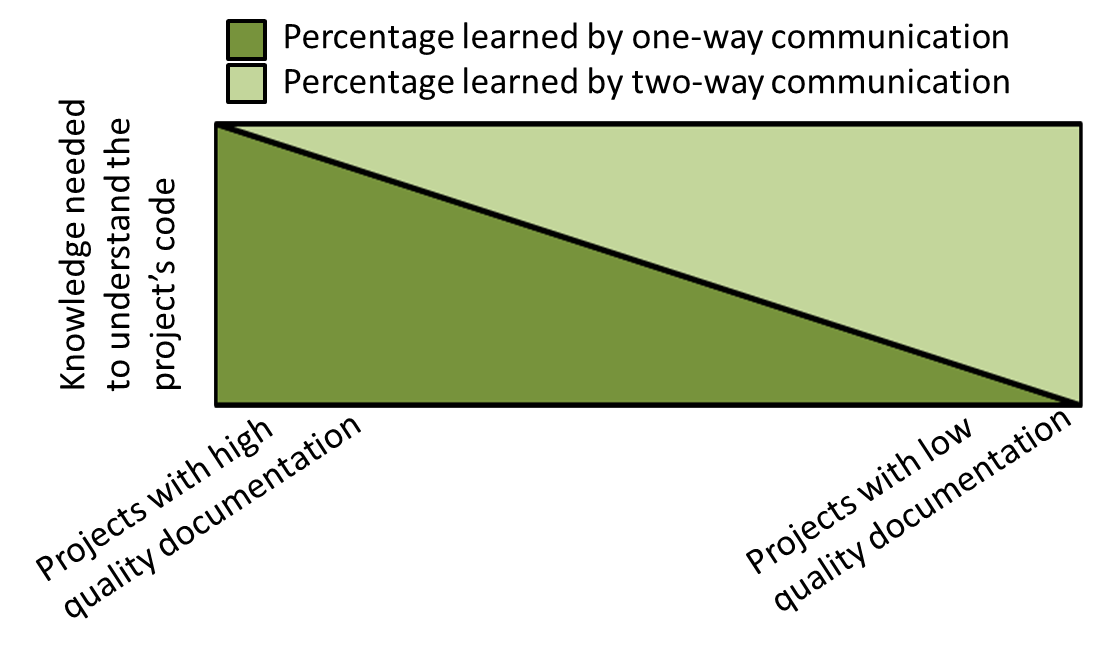
\includegraphics[width=0.85\textwidth]{Graph1}
    \caption{Percentage of one-way and two-way communication required for different types of projects with high and low quality documentation}
    \label{graph1}
\end{figure}






\section{Conclusion}

In my experience working with several different contexts of knowledge transfer in an industrial environment
I can conclude that there are two major ways of transferring knowledge from mentors to newcomers: One-way
and two-way communication. One-way communication is usually perceived in the form of documentation and it 
is characterized by the fact that information flows in only one direction. From my point of view, the most 
important of the several different kinds of documentation, is the internal documentation which encompasses
names of classes, variables, methods and developer written comments. The importance of this comes from
the immediateness of this kind of documentation to satisfy doubts the newcomers may have, and also because
it is the most commonly used documentation by the newcomers. Two-way communication is needed in a inversely 
proportional manner to the quality of said documentation.

Some high level factors that can highly improve the learning experience of newcomers when joining a new software 
project are:
\begin{itemize}
  \item The presence of both documentation and an expert, with emphasis in the former
  \item Knowledgeable and available mentor(s)
  \item As long as possible, include newcomers into already existing teams with an already defined work culture 
\end{itemize}

I can derive from this information that applying best practices from code maintenance literature such as 
using meaningful names for classes, variables and methods in the project's code, and constantly updating
the developer written comments is optimal for the knowledge transfer process in newcomers. Therefore making
the need for two-way communication between newcomers and mentors minimal, which is also advantageous for the
company since mentors tend to be more senior developers and the time that mentors spend mentoring newcomers
is time they are not creating new products or fixing important errors which usually has a high priority
in industrial environments.

 


\bibliographystyle{abbrv}
\bibliography{sigproc}  % sigproc.bib is the name of the Bibliography in this case
% You must have a proper ".bib" file
%  and remember to run:
% latex bibtex latex latex
% to resolve all references

 
\end{document}